\section{Toy-Problem Pilot}
\label{sec:pilot}

% =========================================================================
% Pilot study run on the LLM context MDP scaffold described in Section~\ref{sec:method}.
% Scope is deliberately small: the question is whether the expert-iteration loop
% closes at all under the framework's design, not whether it produces frontier
% accuracy on standardized benchmarks. The latter requires the pre-registered
% study of Section~\ref{sec:experimental-plan}.
% =========================================================================

This section reports a toy-problem pilot conducted on the LLM context MDP
scaffold of Section~\ref{sec:method}. The purpose is narrow and the scope
admits no claim about benchmark performance: we test whether the expert
iteration loop of Section~\ref{sec:method-training} produces measurable
round-over-round improvement on a tiny problem set when implemented
end-to-end, and whether the trained parametric heads transfer to held-out
problems of the same structural shape. The pre-registered benchmark study
of Section~\ref{sec:experimental-plan} is the empirical claim of the
program; what follows is the integration check whose negative outcome
would have falsified the framework's basic feasibility before any
benchmark run.

\subsection{Pilot Setup}
\label{sec:pilot-setup}

The pilot exercises four toy problems sampled to cover four families of
verb-choice difficulty: an arithmetic single-step problem
(\texttt{multiply\_small}: ``Compute $7 \cdot 6$''); a single-step word
problem (\texttt{gsm8k\_toy\_1}: a $3 \cdot 12 - 7$ word problem); a
two-step linear-algebra problem (\texttt{algebra\_toy\_1}: ``Solve
$2x + 5 = 13$''); and a quadratic-factoring problem (\texttt{factor}:
``Factor $x^2 - 9$''). A second set of four structurally parallel
problems, fixed in advance and never used during training, serves as the
held-out evaluation set: a different arithmetic operand pair
(\texttt{multiply\_small\_ho}: ``Compute $9 \cdot 8$''), a different
word problem (\texttt{gsm8k\_toy\_ho}: a $4 \cdot 15 - 9$ word problem),
a different linear-algebra problem (\texttt{algebra\_toy\_ho}: ``Solve
$3y - 7 = 8$''), and a different quadratic to factor
(\texttt{factor\_ho}: ``Factor $x^2 + 5x + 6$''). The held-out set
shares structural shape but never surface content with the training set,
so a model that has memorized verb sequences on training problems will
score poorly on held-out problems if those memorized sequences fail to
generalize.

The base language model throughout the pilot is Qwen2.5-3B running
locally via Ollama; the same model serves both as the verb instantiator
(filling in the textual content of each cognitive verb) and as the
2048-dimensional state encoder. The agent's parametric heads are a
shared encoder of one fully-connected layer of width 512 with
LayerNorm and GELU plus a representation projection of width 256,
feeding a 7-way policy head and a 7-way value head. The total trainable
parameter count is $1.19\mathrm{M}$ on top of a frozen base model.

MCTS is run with a simulation budget of $B = 20$ at every state visited
by a scripted three-step trajectory (\textsc{FormHypothesis},
\textsc{InvokeVerifier}, \textsc{CommitAnswer}). Five MCTS random seeds
are run per problem, producing 15 records per problem and 60 records
per dataset on the four-problem training and held-out sets. The MCTS
discount is $\gamma = 0.99$ and the PUCT exploration constant is
$c_{\PUCT} = 1$. The rollout depth limit is zero, so the leaf
evaluator is the value head when present and a constant zero when
absent. The verifier of Section~\ref{sec:method-reward} is the SymPy
equality call on canonicalized normal forms; correct commits earn
$+1$, incorrect commits earn $-1$, and intermediate verifier calls
on hypotheses earn small shaped rewards as specified in
Section~\ref{sec:method-reward}.

The pilot fits four sets of heads. The \emph{baseline} heads
(denoted \texttt{v2}) are distilled from targets collected under a
uniform PUCT prior: no parametric prior has yet entered the loop, so
these heads are the pre-expert-iteration starting point. The
\emph{first-round} heads (\texttt{v3}) are distilled from targets
collected on the same four problems but with the baseline heads
installed as the PUCT prior; this is the first round of expert
iteration. The \emph{second-round} heads (\texttt{v4}) are distilled
from targets collected with the first-round heads as prior on an
expanded problem set of seven problems (the original four plus three
word-problem variants). The \emph{rebalanced second-round} heads
(\texttt{v4b}) are an alternative second-round fit on a $10$-problem
training set: the same seven problems used by \texttt{v4} plus two
algebra variants and one factoring variant, with composition
$10\%/40\%/30\%/20\%$ (arithmetic/word/algebra/factoring) instead of
\texttt{v4}'s $14\%/57\%/14\%/14\%$. The held-out set is the same
across all rounds, so any generalization shift can be attributed to
the trained heads, not to a shift in evaluation distribution.

\paragraph{Round-naming convention.} Throughout this section we use
\texttt{v2}, \texttt{v3}, and \texttt{v4} as terse labels for the
baseline, first-round, and second-round heads respectively; the
identically-named distillation datasets are the inputs from which each
head set is fitted. Comparisons phrased as ``after one round of expert
iteration'' refer to the \texttt{v2}-to-\texttt{v3} transition;
``after two rounds'' refers to \texttt{v2}-to-\texttt{v4}.

\begin{figure}[t]
\centering
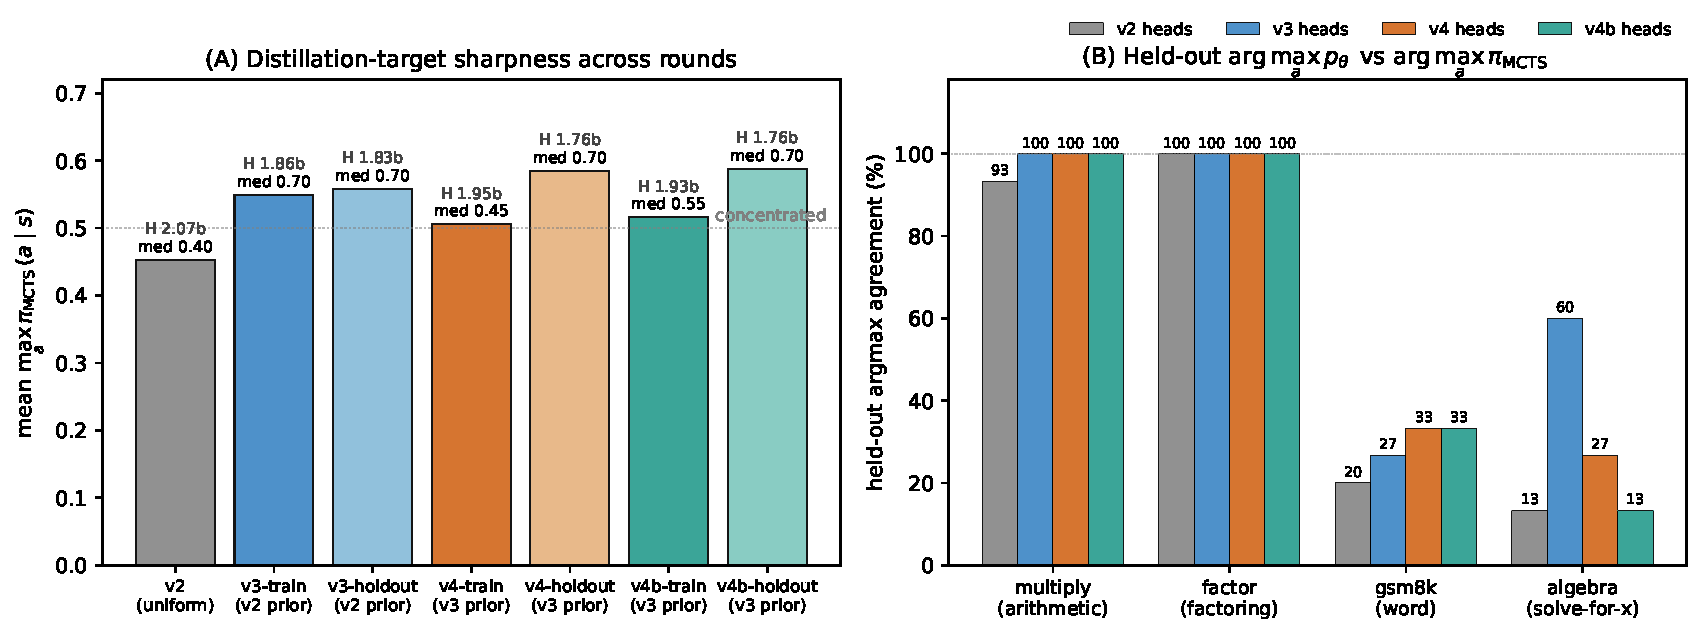
\includegraphics[width=\linewidth]{figures/pilot_results.pdf}
\caption{Headline pilot results. \emph{Panel A:} sharpness of the
$\pimcts$ distillation targets across pilot rounds, reported as mean
$\max_a \pimcts(a \given s)$ per dataset (bar) with the median and
entropy annotated above the bar. The transition from \texttt{v2}
(uniform PUCT prior) to \texttt{v3-train} (trained PUCT prior) is the
intended round-over-round sharpening; \texttt{v3-holdout} confirms the
sharpening generalizes to problems the prior had not seen during
training. \texttt{v4-train}'s lower sharpness reflects the prior
acting near-uniform on three problem variants it had never encountered;
\texttt{v4b-train} sits between \texttt{v4-train} and \texttt{v3-train}
because its larger problem set mixes seen and unseen variants in a
different ratio. \emph{Panel B:} zero-shot held-out argmax agreement on
the canonical \texttt{v3-holdout} evaluation set, defined as
$\arg\max_a \ptheta(a \given s) = \arg\max_a \pimcts(a \given s)$,
broken out by problem family. \texttt{v3} heads improve uniformly over
\texttt{v2} heads; \texttt{v4} heads improve on the targeted word
problem family ($+6.7$ pp) but regress sharply on algebra
($-33.3$ pp). The rebalanced \texttt{v4b} heads hold the word-problem
gain but do not recover algebra despite raising its training share above
the baseline, the controlled test that Section~\ref{sec:pilot-v4b} uses
to rule out class dilution as the dominant regression mechanism.}
\label{fig:pilot-headline}
\end{figure}

\subsection{Baseline to First-Round Heads: Monotonic Improvement}
\label{sec:pilot-v2-v3}

The first round of expert iteration demonstrates the loop closing on
every metric simultaneously, summarized graphically in
Figure~\ref{fig:pilot-headline}. This subsection reports three families
of measurement, and each tightens from the baseline to the first-round
heads: the sharpness of the MCTS distillation targets, the
training-loss floor of the distilled heads, and zero-shot held-out
generalization. Table~\ref{tab:pilot-sharpness} reports
the sharpness of the MCTS visit-count targets $\pimcts$ across rounds.
The targets become measurably sharper from \texttt{v2} (uniform prior)
to \texttt{v3-train} (trained prior): mean maximum probability rises
from $0.452$ to $0.549$, median maximum from $0.40$ to $0.70$, and
entropy drops by $0.215$ bits. The held-out collection \texttt{v3-holdout}
is similarly sharp despite using problems never seen during training,
which is consistent with the prior generalizing structurally rather
than overfitting surface content.

\begin{table}[t]
\centering
\caption{Sharpness of $\pimcts$ targets across pilot rounds.
``mean max'' is the mean over records of $\max_a \pimcts(a \given s)$;
``med max'' is the median; entropy is in bits; ``frac concentrated''
counts records with maximum at least $0.5$.}
\label{tab:pilot-sharpness}
\small
\begin{tabular}{@{}lrrrrr@{}}
\toprule
Dataset & $N$ & mean max & med max & entropy & frac $\geq 0.5$ \\
\midrule
\texttt{v2}                  (uniform, 4 problems)    & 60  & 0.452 & 0.400 & 2.070 & 35\% \\
\texttt{v3-train}            (v2 prior, 4 problems)   & 60  & 0.549 & 0.700 & 1.855 & 62\% \\
\texttt{v3-holdout}          (v2 prior)               & 60  & 0.558 & 0.700 & 1.833 & 63\% \\
\texttt{v4-train}            (v3 prior, 7 problems)   & 105 & 0.506 & 0.450 & 1.945 & 49\% \\
\texttt{v4-holdout}          (v3 prior)               & 60  & 0.585 & 0.700 & 1.762 & 68\% \\
\texttt{v4b-train}           (v3 prior, 10 problems)  & 150 & 0.516 & 0.550 & 1.927 & 53\% \\
\texttt{v4b-holdout}         (v3 prior)               & 60  & 0.588 & 0.700 & 1.756 & 72\% \\
\bottomrule
\end{tabular}
\end{table}

The sharper targets translate into a lower training-loss floor for the
distilled heads. Table~\ref{tab:pilot-training} reports the final
policy cross-entropy (in nats) and value mean-squared-error after $200$
full-batch Adam epochs at learning rate $10^{-3}$ on each round's
dataset. The \texttt{v3} heads converge to a final policy CE of $1.29$
nats against \texttt{v2}'s $1.45$ nats, a relative reduction of $10.9\%$; the
$Q$-MSE drops by $39.1\%$. The lower CE floor is a direct consequence
of lower target entropy: cross-entropy against a target distribution
is bounded below by the entropy of the target (here $1.855$ bits
$\approx 1.286$ nats for \texttt{v3-train}), and sharper targets
relax this lower bound. Training-set argmax agreement, defined as the
fraction of records on which $\arg\max_a \ptheta(a \given s)$ matches
$\arg\max_a \pimcts(a \given s)$, rises from $85.0\%$ to $91.7\%$.

\begin{table}[t]
\centering
\caption{Training-time fit of the distilled heads across pilot rounds.
``Training argmax'' is the fraction of records on which the trained
policy's argmax agrees with the MCTS visit-count argmax on the same
dataset.}
\label{tab:pilot-training}
\small
\begin{tabular}{@{}lrrr@{}}
\toprule
Round & Final policy CE (nats) & Final $Q$-MSE & Training argmax \\
\midrule
\texttt{v2}   & 1.4512 & 0.006829 & 85.0\% \\
\texttt{v3}   & \textbf{1.2934} & \textbf{0.004156} & \textbf{91.7\%} \\
\texttt{v4}   & 1.3574 & 0.005477 & 88.6\% \\
\texttt{v4b}  & 1.3501 & 0.005348 & 88.7\% \\
\bottomrule
\end{tabular}
\end{table}

The held-out generalization figures, summarized in
Table~\ref{tab:pilot-holdout}, are the headline pilot result. The
\texttt{v3} heads evaluated zero-shot on \texttt{v3-holdout} achieve
$71.7\%$ argmax agreement with the held-out MCTS targets, against the
\texttt{v2} heads' $56.7\%$ on the same data. This is a $15.0$
percentage-point absolute improvement after a single round of expert
iteration (single training seed; cf.~Section~\ref{sec:pilot-caveats}),
and the mean $L_1$ distance between $\ptheta$ and $\pimcts$ falls
from $0.540$ to $0.314$, a $42\%$ relative reduction.
The improvement is uniform across problem families: every problem in
the held-out set improves or holds at $100\%$ from \texttt{v2} to
\texttt{v3}.

\begin{table}[t]
\centering
\caption{Held-out generalization on \texttt{v3-holdout} ($60$ records,
$4$ problems, $5$ seeds each). Argmax agreement is $\ptheta$'s argmax
versus $\pimcts$'s argmax; mean $L_1$ is the $L_1$ distance between
$\ptheta$ and $\pimcts$ averaged over records. Single training seed
per head; cf.~Section~\ref{sec:pilot-caveats}.}
\label{tab:pilot-holdout}
\small
\begin{tabular}{@{}lrrrr@{}}
\toprule
Problem & \texttt{v2} agree & \texttt{v3} agree & \texttt{v4} agree & \texttt{v4b} agree \\
\midrule
\texttt{multiply\_small\_ho}  &  93.3\% & 100\%   & 100\%   & 100\%   \\
\texttt{factor\_ho}           & 100\%   & 100\%   & 100\%   & 100\%   \\
\texttt{gsm8k\_toy\_ho}       &  20.0\% &  26.7\% &  33.3\% &  33.3\% \\
\texttt{algebra\_toy\_ho}     &  13.3\% &  60.0\% &  26.7\% &  13.3\% \\
\midrule
\textbf{Overall}              & 56.7\%  & \textbf{71.7\%} & 65.0\%  & 61.7\%  \\
\textbf{Mean $L_1$}           & 0.540   & \textbf{0.314}  & 0.407   & 0.347   \\
\bottomrule
\end{tabular}
\end{table}

\subsection{First-Round to Second-Round Heads: A Targeted Intervention with Collateral Damage}
\label{sec:pilot-v3-v4}

The weakest generalization point after the first round is
\texttt{gsm8k\_toy\_ho} at $26.7\%$ argmax agreement, a quantitative
expression of the qualitative observation that the word problem
family carries more verb-choice ambiguity than the arithmetic or
factoring families. The intuitive intervention is to add word-problem
variants to the training set so that the heads see more examples of
the family they handle worst. The second-round fit (\texttt{v4})
therefore expands the training problem set from four problems to seven
by adding three new word-problem variants with different surface
content and different numerical answers, and re-collects targets with
the first-round heads as the MCTS prior.

The intervention produced the targeted gain on word problems
(\texttt{gsm8k\_toy\_ho} argmax agreement rises from $26.7\%$ to
$33.3\%$, a $6.7$ percentage-point improvement) at the cost of a
$33.3$ percentage-point regression on the algebra family
(\texttt{algebra\_toy\_ho} falls from $60.0\%$ to $26.7\%$). The net
effect on aggregate held-out argmax agreement is negative
(Table~\ref{tab:pilot-holdout}), and the mean $L_1$ to the held-out
targets rises by $0.093$. The framework's first round of expert
iteration produced a measurable improvement; the second round, with a
naively-expanded training set, produced a measurable regression on a
problem family that was not the target of the intervention.

The regression is structurally informative. Three independent
mechanisms contribute, surfaced by a post-mortem comparison of the
\texttt{v3}-train and \texttt{v4}-train algebra targets and a
side-by-side comparison of \texttt{v3} and \texttt{v4} head predictions
on the held-out algebra records.

\paragraph{Class dilution.} The four-problem training set used for the
baseline and first-round head fits was perfectly balanced ($25\%$ per
family). The seven-problem training set used for the second-round head
fit has composition $14.3\%$ arithmetic, $57.1\%$ word problems,
$14.3\%$ algebra, $14.3\%$ factoring. Adding three problems of one
family while leaving the others fixed reduced the relative weight of
every other family by $43\%$ (from $25.0\%$ to $14.3\%$). Because the
algebra family carries the highest verb-choice ambiguity in the toy
set, it is the most sensitive to a reduction in its training share.

\paragraph{Target instability.} Matched MCTS seeds across collection
runs do not produce the same $\pimcts$ targets on the algebra family.
The cleanest comparison holds the prior fixed: the \texttt{v4}-train
and \texttt{v4b}-train collections (the latter from the rebalancing
experiment of Section~\ref{sec:pilot-v4b}) both used the first-round
heads as the PUCT prior on \texttt{algebra\_toy\_1} with the same five
MCTS seeds, yet the mean $L_1$ distance between their targets at
matched (seed, turn) pairs is $0.553$, with only $7$ of $15$ records
agreeing on the argmax verb. (Across rounds with different priors,
\texttt{v3}-train versus \texttt{v4}-train, the corresponding figures
are $0.633$ and $7/15$; the prior change adds little on top of the
sampling noise.) The randomness source is the environment itself: the
MCTS seed controls action selection inside the search, but the LLM
transitions are sampled at temperature $0.7$ without a fixed sampling
seed, so each collection run draws different continuations. The
non-reproducibility is also state-dependent in an informative way.
On the held-out algebra problem, whose states at turn $\geq 1$ are
dominated by a terminal commit with a deterministic verifier reward,
the \texttt{v4}-holdout and \texttt{v4b}-holdout collections (same
prior, same seeds) reproduce almost exactly: mean $L_1 = 0.087$ with
$14/15$ argmax agreement. On the training algebra states, where
several verbs are genuinely competitive and their sampled returns
overlap, the targets do not reproduce. Instability concentrates
exactly where verb choice is ambiguous, which is where the
target-stability metric of Section~\ref{sec:pilot-lessons} needs to
look. The first-round heads were trained on one particular
realization of this target noise; the second-round heads were trained
on a different realization. The candidate cure is a larger simulation
budget, so that the visit-count estimator concentrates on the
high-value verb before the trajectory is committed. We test that cure
directly in Section~\ref{sec:pilot-bsweep}: it works, agreement between
independent collections rises steadily with budget, and the pilot's
$B = 20$ turns out to sit at the low-agreement floor of the measured
curve.

\paragraph{Brittle shortcut exploitation.} Step-by-step inspection of
the first-round heads' predictions on held-out algebra records
reveals a structural shortcut that the head-fitting has picked up.
On the ten held-out algebra records at turn $\geq 1$, the
first-round heads predict \textsc{CommitAnswer} on $9/10$ ($90\%$);
the second-round heads predict \textsc{CommitAnswer} on $2/10$
($20\%$) and predict \textsc{ComputeSubexpr} on $6/10$ ($60\%$). The
first-round shortcut matches algebra's first-round MCTS targets
(which also concentrate on \textsc{CommitAnswer} after one or two
turns in five of five seeds) and produces strong per-turn agreement
in exactly that turn band ($\arg\max$ agreement with the held-out
MCTS targets at turn $1$ is $4/5 = 80\%$ for the first-round heads
and $0/5$ for the second-round heads; at turn $2$ it is
$5/5 = 100\%$ for the first round and $2/5 = 40\%$ for the second).
The second-round training set added word-problem variants in which
the correct verb at turn $1$ is \textsc{ComputeSubexpr} rather than
\textsc{CommitAnswer}, so the second-round heads broke the
``commit at turn $1$'' shortcut. The shortcut's collapse improves
the model genuinely on word problems and harms the model on algebra,
where the shortcut had been load-bearing. The trade-off is between a
brittle pattern that happened to work on one family and a more
general pattern that works on a different family.

\subsection{Testing the Class-Balance Hypothesis: \texttt{v4b}}
\label{sec:pilot-v4b}

The post-mortem of Section~\ref{sec:pilot-v3-v4} offered three
candidate mechanisms for the algebra regression. Two of them
(target instability, brittle shortcut exploitation) are observational
findings that the pilot's data already supports. The third (class
dilution) is a falsifiable hypothesis that the pilot can test directly
by re-running the second-round head fit on a deliberately rebalanced
training set. We carried out that test as \texttt{v4b}.

\paragraph{Setup.} The \texttt{v4b} training set adds three problems
to the seven-problem \texttt{v4} set: two algebra variants
(\texttt{algebra\_toy\_2}: ``Solve $4x - 3 = 9$''; \texttt{algebra\_toy\_3}:
``Solve $7x + 2 = 16$'') and one factoring variant
(\texttt{factor\_2}: ``Factor $x^2 - 16$''). The composition shifts
from $14.3\%/57.1\%/14.3\%/14.3\%$ to
$10\%/40\%/30\%/20\%$ (arithmetic/word/algebra/factoring). Crucially,
algebra's share recovers from $14\%$ to $30\%$, slightly above
\texttt{v4}'s and the baseline's $25\%$. Every other parameter is
held fixed: same first-round (\texttt{v3}) heads as prior, same MCTS
budget $B = 20$, same five MCTS seeds, same head architecture, same
$200$-epoch Adam training. If class dilution were the dominant
mechanism behind the \texttt{v3}-to-\texttt{v4} algebra regression,
rebalancing should restore algebra performance closer to
\texttt{v3}'s level.

\paragraph{Result.} It does not. \texttt{v4b}'s algebra held-out
argmax agreement falls to $13.3\%$
(Table~\ref{tab:pilot-holdout}), \emph{below} both \texttt{v4}'s
$26.7\%$ and \texttt{v3}'s $60.0\%$. Mean $L_1$ on algebra
\emph{improves} ($0.823$ for \texttt{v2}, $0.356$ for \texttt{v3},
$0.868$ for \texttt{v4}, $0.758$ for \texttt{v4b}), so
\texttt{v4b}'s algebra predictions are closer to the held-out
targets in distance even though the argmax does not match. The
overall held-out argmax agreement of \texttt{v4b} is $61.7\%$
($37/60$), between \texttt{v4} ($65.0\%$) and \texttt{v3} ($71.7\%$);
overall mean $L_1$ is $0.347$, the second-best across rounds after
\texttt{v3}'s $0.314$. The targeted gain on word problems holds
(\texttt{gsm8k\_toy\_ho} stays at $33.3\%$). The training-set fit
moves slightly toward \texttt{v3}'s floor (CE $1.350$ vs \texttt{v4}'s
$1.357$ and \texttt{v3}'s $1.293$).

\paragraph{Interpretation.} \texttt{v4b} is a rebalance-plus-expansion
rather than a pure rebalance: it both raises algebra's training share
and enlarges the set with three fresh instances (two algebra, one
factoring), so it gives algebra more absolute data as well as a larger
relative share. This strengthens the refutation rather than weakening
it: the class-dilution mechanism, taken
alone, predicts that rebalancing (let alone adding fresh algebra
instances) recovers algebra. Rebalancing did
not recover algebra, so class dilution is not the dominant mechanism
behind the \texttt{v3}-to-\texttt{v4} algebra regression at the
pilot's scale. The two remaining candidates from
Section~\ref{sec:pilot-v3-v4} therefore become the leading
explanation. Target instability predicts that algebra's MCTS
visit-count distributions at $B = 20$ are too noisy across collection
runs for distillation to lock onto the algebra-correct pattern; this
is confirmed by the same-prior comparison reported in
Section~\ref{sec:pilot-v3-v4}: the \texttt{v4}-train and
\texttt{v4b}-train collections, identical in prior, problems, and MCTS
seeds, produce \texttt{algebra\_toy\_1} targets with mean
$L_1 = 0.553$ and only $7/15$ argmax agreement. Brittle-shortcut breakage predicts
that any second-round head fit (whether or not the training set is
rebalanced) loses the ``commit at turn $\geq 1$'' shortcut that
\texttt{v3} happened to learn; on the held-out \texttt{algebra\_toy\_ho}
records at turn $\geq 1$, the rebalanced \texttt{v4b} heads predict
\textsc{CommitAnswer} on $2/10$ ($20\%$), identical to \texttt{v4}'s
rate and well below \texttt{v3}'s $9/10$ ($90\%$), confirming the
shortcut is broken regardless of the rebalance. Neither of these mechanisms is class-balance-sensitive,
and the pilot's data is consistent with both being at work
simultaneously.

\paragraph{What the test refutes and what it does not.} \texttt{v4b}
refutes the strong claim that the algebra regression is a class-balance
problem fixable by class-balance correction. It does not refute the
broader monitoring commitment that the discussion of
Section~\ref{sec:pilot-lessons} draws from the \texttt{v3}-to-\texttt{v4}
result. Reporting per-class composition and per-class held-out accuracy
is still required to distinguish mechanism from anomaly in any
multi-round expansion. The \texttt{v4b} result simply moves the leading
hypothesis from class composition to target stability and
shortcut-pattern dependence, both of which the pre-registered study's
monitoring protocol (Section~\ref{sec:pilot-lessons}) can detect.

\subsection{What Stabilizes the Distillation Target?}
\label{sec:pilot-bsweep}

The target-instability finding of Section~\ref{sec:pilot-v3-v4} admits
two candidate cures: make the individual LLM transitions reproducible,
or make the visit-count estimator that aggregates them less noisy. We
tested both, and the search budget is what stabilizes the target. For a
fixed initial state we ran $K = 20$ independent MCTS searches (different
random seeds, hence independent stochastic LLM transitions) at every
budget $B \in \{10, 20, 40, 80, 160\}$ on \texttt{multiply\_small} (a
low-ambiguity control) and \texttt{algebra\_toy\_1} (the high-ambiguity
family). Holding the start state fixed isolates the visit-count
estimator's own sampling variance from the trajectory cascade. The
stability statistic is \emph{pairwise argmax agreement}: the probability
that two independent searches recommend the same verb, over all
$\binom{20}{2} = 190$ pairs, with bootstrap confidence intervals.

The result is that \emph{agreement rises with budget, and the pilot's
$B = 20$ sits at the low-agreement floor}: pairwise agreement climbs from
$0.31$--$0.32$ at $B = 20$ to $0.81$ on the easy family and $0.73$ on the
hard family at $B = 160$, with sharpness (mean max-probability) rising in
lockstep. At the budget the pilot actually collected with, two
independent collections agree on the training argmax less than a third of
the time, so the pilot's observed target instability is an expected
property of its budget rather than an indictment of the framework, and it
supports paying for the pre-registered heavy-search budget. Two
measurement lessons carry into the larger study. First, \emph{mean $L_1$
between visit-count distributions is the wrong stability metric}: it is
confounded by sharpness and on the hard family rises monotonically with
budget even as true stability also rises, so the earlier $L_1$ figures in
this section (such as the $0.553$ on matched-condition algebra at
$B = 20$) mix genuine disagreement with this artifact, and \emph{pairwise
recommended-verb argmax agreement} is the correct signal. Second,
convergence speed is family-dependent (the easy family reaches $0.73$ by
$B = 80$, the hard family needs $B = 160$), so the heavy-search budget
must be set by the slowest-converging family, and the agreement
diagnostic reported \emph{stratified by problem family} rather than
pooled. The full budget--stability table
(Table~\ref{tab:pilot-bsweep}), the curves (Figure~\ref{fig:pilot-bsweep}),
the negative per-call-seeding result, and the $K = 6$-versus-$K = 20$
small-sample artifact are in Appendix~\ref{app:bsweep}.

\subsection{Closing the Loop End-to-End (Run In Progress)}
\label{sec:pilot-closedloop}

The experiments above isolate one step of the framework: they collect MCTS
targets once and distill them into the heads in a single offline pass per
round. The full method of Section~\ref{sec:method-training} is an online loop.
Search with the current heads as the PUCT prior and the target-$Q$ head as the
bootstrap leaf value, distill the resulting $\pimcts$ and $\Qmcts$ into the
heads, then re-prior the next round of search with the updated heads. We have
now implemented that loop and begun running it. This subsection reports the
implementation and the infrastructure-level results that are already in, and is
explicit that the central learning-signal result is pending a run that is
executing as we write.

\paragraph{In-process frozen model and a faithful state embedding.}
The pilot ran against an Ollama HTTP server and read its embedding endpoint for
the $2048$-dimensional state vector. That endpoint regressed after a server
upgrade (Section~\ref{sec:pilot-reproducibility}), and an HTTP endpoint can in
any case neither expose the base model's hidden state, which the adapter
architecture of Section~\ref{sec:method-architecture} requires, nor make the
decoder forwards countable for compute accounting. We therefore moved the
frozen model in process. The state embedding is now $\mathrm{embed}(s) = h_T$,
the last-layer hidden state at the sentinel position
(Section~\ref{sec:method-architecture}), taken from the same weights that
generate verb content rather than from a separate endpoint. On a $1.5$B
substrate this was verified to give seeded-generation reproducibility, a
deterministic masked-mean hidden-state pooling, countable per-decision decoder
forwards, and a single frozen copy in memory serving both the encoder and the
generator roles.

\paragraph{One forward per decision.}
Section~\ref{sec:method-architecture} specifies that a single state prefill
should serve both the heads and verb generation (``one forward, not two''). We
implemented this as a shared encoder that prefills the verb-independent state
prefix once, returning both $h_T$ and the key-value cache that seeds every
verb's generation. Against a real $1.5$B model the shared prefill reproduces a
standalone forward's $h_T$ to bit identity and produces token-identical greedy
generation under single precision; under \texttt{bfloat16} an occasional final
token differs, which is the reduction-order compute floor that the budget sweep
of Section~\ref{sec:pilot-bsweep} already identified rather than a logic error.
For a four-verb node the shared prefill cuts prefilled tokens by about $53\%$
relative to re-encoding the full state once per verb, and the saving grows with
state length and branching factor.

\paragraph{The training loop of Section~\ref{sec:method-training}.}
We implemented the combined objective
$L_{\mathrm{total}} = L_Q + \lambda L_{\pi}$, in which $L_Q$ is a masked
mean-squared error of $\Qpsi$ against the MCTS chance-node estimate $\Qmcts$
(the framework's stated target, not a single-sample bootstrapped Bellman
target) and $L_{\pi}$ is the masked cross-entropy of the policy head against
the visit-count distribution $\pimcts$, together with the prioritized replay
buffer and the periodically-synced target-$Q$ network. On the pilot's own
\texttt{v2} records this objective drives $L_Q$ down by about an order of
magnitude (from $0.111$ to $0.012$ over $400$ steps) while $L_{\pi}$ settles at
about $1.46$, matching the pilot's \texttt{v2} final policy cross-entropy of
$1.4512$ (Section~\ref{sec:pilot-v2-v3}). The new architecture and loop thus
reproduce the pilot's distillation behavior on identical data while adding the
replay and target-network machinery that the pilot performed by hand across
sessions or not at all.

\paragraph{A first closed-loop run and its compute cost.}
We then ran the full online loop on a GPU for three iterations over the four
training families, $200$ training steps per iteration. The substrate was a
$1.5$B model at the parameter scale of the pre-registered plan, though an
instruct-and-math-specialized variant chosen for feasibility rather than the
base-only substrate the pre-registered study mandates for clean attribution
(Section~\ref{sec:exp-models}); the closed-loop observations here are therefore
feasibility evidence, not a substrate-faithful result. The run's headline
number is the honest per-decision compute cost. Averaged over the $96$
decisions, each decision cost about $27$ verb generations and roughly $9000$
generated tokens against a single state prefill of about $114$ tokens.
Generation dominates the decision's compute by about $79$ to $1$ in tokens, and
the prefill count of about one per decision confirms that the
one-forward-per-decision property of Section~\ref{sec:method-architecture}
holds in practice and not only by construction. This is the per-decision
measurement on which the FLOP-accounted compute axis of the pre-registered plan
(Section~\ref{sec:exp-compute}) is built.

\paragraph{Observability is load-bearing, and the pending result.}
The first run persisted only a per-iteration loss summary, and in that summary
$L_{\mathrm{total}}$ is dominated by $L_{\pi}$ sitting near its target-entropy
floor of about $1.4$ (the same floor as the pilot's $1.4512$), so the small
$L_Q$ term and the prior-sharpening dynamic were not separately visible: the
two signals that Section~\ref{sec:method-training} predicts could not be read
off a fourteen-hour run. We rebuilt the run harness so that a long run is both
observable and recoverable. It records, per iteration, the separated $L_Q$ and
$L_{\pi}$, the Shannon entropy of the visit distribution $\pimcts$ and of the
learned prior $\ptheta$ over the iteration's decisions (the sharpening
diagnostic, where lower entropy means more concentrated search), and the
per-decision FLOP counters, and it checkpoints after every trajectory so an
interrupted run resumes from its last checkpoint rather than restarting. The
prior-entropy read reuses the cached state prefill and so does not perturb the
compute accounting.

The first end-to-end run of this fully instrumented loop is executing as we
write, five iterations over the toy families. Its learning-signal results, the
across-iteration $L_Q$ trend predicted by approximate $Q$-learning and the
sharpening of $\ptheta$ and of the search visits predicted by expert iteration
(Section~\ref{sec:method-training}), are pending and will be reported when the
run completes. The order-of-magnitude $L_Q$ decrease on the pilot's data above,
and the single-round generalization gain of Section~\ref{sec:pilot-v2-v3}, are
existing evidence that the objective and the distillation step each work in
isolation; the in-progress run is the first test of whether those signals
persist across iterations of the closed online loop. It is the most important
experiment we have conducted for the framework's central dynamic, and we state
plainly that its result is not yet in.

\subsection{Lessons for the Pre-Registered Study}
\label{sec:pilot-lessons}

Three of the pilot's findings carry directly into the larger study.

First, the improvement from baseline to first-round heads is evidence
that the expert-iteration loop closes under the framework's
implementation: distilling sharper MCTS targets into the parametric
heads produces measurable generalization gains on held-out problems
of the same structural shape, exactly as
Section~\ref{sec:method-training} predicts. This validates the
integration of the framework's components (the LLM context MDP, the
verifier-anchored reward, the shared-encoder architecture, MCTS as a
policy improvement operator) end-to-end, independently of whether the
pre-registered benchmark study eventually finds a positive
compute-versus-accuracy frontier.

Second, the regression from first-round to second-round heads, and
the \texttt{v4b} test that rules out class dilution as the dominant
mechanism, together suggest that the operative limit at the pilot's
scale is target stability and shortcut-pattern dependence rather than
training-set composition alone. The per-round training-set composition
is still a design parameter inside our pipeline and worth tracking,
but the pilot now identifies more upstream concerns: the across-seed
$L_1$ of $\pimcts$ on high-ambiguity states at $B = 20$, and the
implicit patterns that head fits exploit when the training set is
small. We pre-commit to reporting both per-class composition and a
target-stability diagnostic alongside any multi-round results in the
benchmark study, so that a future regression of the same shape is
attributable to mechanism rather than misread as a framework failure.

Third, the budget sweep of Section~\ref{sec:pilot-bsweep} turns the
target-instability finding from a hypothesis into a measured trend: the
pilot's $B = 20$ sits at the low-agreement floor of the
budget--stability curve (pairwise argmax agreement $0.31$--$0.32$
across independent collections), and agreement rises with budget to
$0.81$ on the easy family and $0.73$ on the hard family at $B = 160$
($K = 20$ searches per cell, bootstrap CIs in
Table~\ref{tab:pilot-bsweep}). This both supports the pre-registered
heavy-search budget $B = 500$ and changes how we will measure
stability. Because mean $L_1$ between visit-count distributions is
confounded by sharpness (on the hard family it rises monotonically
with budget while true stability also rises, anti-correlating with the
quantity it is meant to track), the pre-registered target-stability
diagnostic is the \emph{pairwise recommended-verb agreement} across
independent searches from a fixed state, reported on a stratified
sample of training states per benchmark and \emph{stratified by
problem family} rather than pooled. Agreement below a pre-committed
threshold at the chosen budget is a precondition for trusting any
round-over-round improvement claim, and the budget is set by the
slowest-converging family rather than the average.
\textcolor{red}{\textbf{[PRE-REG TODO: commit the numerical
target-stability threshold; suggested: pairwise recommended-verb
agreement $\geq 0.70$ at the collection budget, stratified by problem
family, confirm]}} The closed-loop harness of
Section~\ref{sec:pilot-closedloop} already records this diagnostic, the entropy
of $\pimcts$ and of $\ptheta$ per iteration, so the benchmark study inherits the
monitoring by construction rather than retrofitting it onto a long run.

\subsection{Caveats}
\label{sec:pilot-caveats}

The pilot is not a benchmark study. The training sets (four to ten
problems across rounds) are small enough that overfitting is the
dominant failure mode rather than underfitting, and the held-out set,
while constructed to share structural shape, contains only four
problems. The simulation
budget $B = 20$ is well below the pre-registered $B = 50$ and $B = 500$.
The base model (Qwen2.5-3B) is larger than the $1.5$B substrate of the
pre-registered plan, and is run via Ollama rather than the production
inference stack of the benchmark study. The pilot makes no
claim about absolute accuracy on GSM8K, MATH, or any other benchmark,
nor about whether the framework's compute-versus-accuracy frontier
clears the pre-registered falsification bar. What the pilot establishes
is feasibility: every component of Section~\ref{sec:method} can be
implemented and the loop, when implemented, behaves the way
Section~\ref{sec:method-training} predicts on the families where the
prediction is sharp. The closed-loop run of
Section~\ref{sec:pilot-closedloop} carries its own caveats: it uses an
instruct-and-math-specialized $1.5$B variant rather than the base-only
substrate of Section~\ref{sec:exp-models}, and its across-iteration learning
signals are pending a run still in progress, so its present contribution is the
implemented loop and the per-decision compute accounting, not a closed-loop
accuracy claim.

\subsection{Reproducibility}
\label{sec:pilot-reproducibility}

The pilot's artifacts are released alongside this paper for independent
verification. The release contains the collection script
(\path{experiments/collect_distillation.py}), the head architecture
(\path{src/verifier_anchored_rl/heads.py}), the head-training script
(\path{experiments/train_heads.py}), the round-comparison
analyzer (\path{experiments/analyze_distillation_rounds.py}), and
the budget-sweep probe of Section~\ref{sec:pilot-bsweep}
(\path{experiments/b_sweep_stability.py}), all
under an open-source licence in the companion repository. Each
distillation dataset (\texttt{v2}, \texttt{v3-train}, \texttt{v3-holdout},
\texttt{v4-train}, \texttt{v4-holdout}, \texttt{v4b-train},
\texttt{v4b-holdout}) is a JSONL file with one record
per (problem, seed, turn) triple, containing the serialized state, the
available verb set, the MCTS visit counts, the chance-node $Q$
estimates, the recommended verb, and the 2048-dimensional embedding
fetched at collection time. The trained head checkpoints
(\path{heads_v2.pt}, \path{heads_v3.pt}, \path{heads_v4.pt},
\path{heads_v4b.pt})
are PyTorch state dictionaries that the released loader script
(\path{src/verifier_anchored_rl/trained_prior.py}) instantiates
into the architecture above. Every random seed used (MCTS seeds $0$
through $4$ per problem; training seed $0$ for the heads) is logged in
the per-record artifacts and in the training-history JSON dumps. The
hyperparameters are summarized in Section~\ref{sec:pilot-setup}; the
companion repository's \path{experiments/results/} directory contains
the full metric dumps. The pilot is reproducible end-to-end on a single
machine with the Qwen2.5-3B model available through any
OpenAI-compatible inference endpoint (the release defaults to Ollama).

The closed-loop extension of Section~\ref{sec:pilot-closedloop} is released
alongside it: the in-process model backend
(\path{src/verifier_anchored_rl/transformers_client.py}), the shared
single-forward encoder (\path{shared_forward.py}), the training loop with
its prioritized replay buffer and target-network sync (\path{train.py},
\path{replay.py}, \path{architecture.py}), the outer-loop orchestration
(\path{outer_loop.py}), and the run harness
(\path{experiments/run_outer_loop.py}), which writes each run to a
self-contained directory carrying full provenance metadata, the per-iteration
metrics above (the separated $L_Q$ and $L_{\pi}$, the visit- and
prior-distribution entropies, and the FLOP counters), the streamed collection
records, and a checkpoint from which an interrupted run resumes. Unlike the
pilot, the closed loop runs the frozen model in process and depends on no
external inference endpoint.
